\section{Tutorial -- Creating a Flowsheet with Linked Simulations}\label{tutorial.sim.flowsheet}


This tutorial is referenced by other tutorials. \textbf{Save the flowsheet in a convenient location for future use.} 

This tutorial demonstrates how to link simulations to nodes, and how to connect nodes in a flowsheet.
Two models are used: (1) a bubbling fluidized bed model in ACM and (2) a cost of electricity (COE) model in Excel. The COE model estimates the cost of electricity for a 650 MW (net before adding capture) supercritical pulverized coal power plant with solid sorbent post combustion CO$_2$ capture process added.

Before starting the tutorial, see Section \ref{tutorial.example.files} to locate and copy the example files to a convenient location.

\begin{enumerate}
	\item Start FOQUS. The Session window displays (Figure \ref{fig.tut.opt.session}).
	\item Enter ``BFB\_opt'' in \bu{Session Name} (without quotes).
	\item Click the \bu{Description} tab. The problem description box displays and is shown in (Figure \ref{fig.tut.opt.description}).
	\item In the problem description box enter information about the problem being solved in the FOQUS session; this information can be more extensive than what is shown in the example.
	\item Save the session file. Click \textbf{\underline{Save Session}} from the \textbf{\underline{Session}} drop-down menu. Enter change log information and a file name when prompted. The \textbf{\underline{Creation Time}} in metadata page will be the time the session is first saved.  The \textbf{\underline{Modification Time}} will be the last time the session was saved. The \textbf{\underline{ID}} is a unique identifier that changes each time the user saves the simulation. The \textbf{\underline{Change Log}} tab provides a record of the changes made each time the session is saved.
\end{enumerate}

\begin{figure}[H]
	\begin{center}
		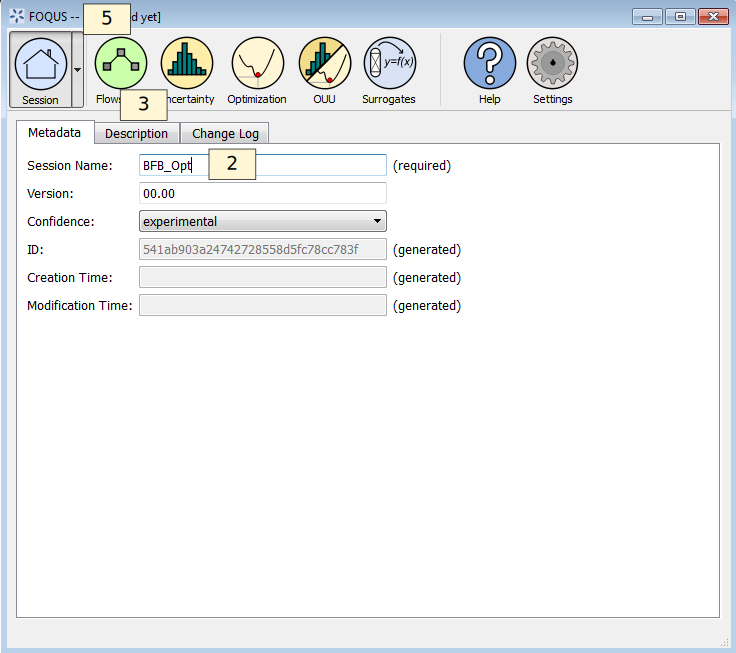
\includegraphics[scale=0.55]{Chapt_flowsheet/figs/session}
		\caption{Session Setup}
		\label{fig.tut.opt.session}
	\end{center}
\end{figure}

\begin{figure}[H]
	\begin{center}
		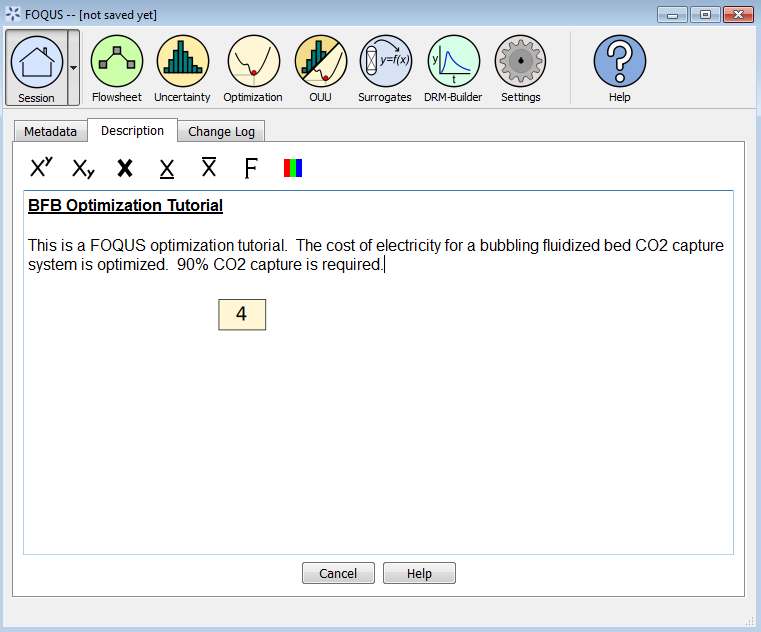
\includegraphics[scale=0.55]{Chapt_flowsheet/figs/description}
		\caption{Session Description}
		\label{fig.tut.opt.description}
	\end{center}
\end{figure}

\label{subsec.opt.tutorial.flowsheet}
There are two models needed for this optimization problem: (1) the ACM model for the BFB capture system and (2) the Excel cost estimating spreadsheet. These models are provided in the example files directory, under optimization/models (see Section \ref{tutorial.example.files}). There are two SimSinter configuration files: (1) BFB\_sinter\_config\_v6.2.json for the process model and (2) BFB\_cost\_v6.2.3.json for the cost model. The next step is to upload the models to Turbine.

\begin{enumerate}
	\setcounter{enumi}{5}
	\item Open the \bu{Add\bs Update Model to Turbine} dialog box (Figure \ref{fig.tut.opt.menu.upload}).
	\item In this case, the SimSinter configuration files have already been created. If a SimSinter configuration file needs to be created for the simulation, \bu{Create/Edit} displays the SimSinter configuration GUI (see Figure \ref{fig.tut.opt.upload}). See the SimSinter documentation or Chapter \ref{chapt.simsinter} for more information.
	\item Click \bu{Browse} to select a SimSinter configuration file (Figure \ref{fig.tut.opt.upload}). Once the SimSinter configuration file is selected, the simulation file and sinterconfig file is automatically added to the files to upload. The application type is entered automatically. If there are additional files required for the simulation, those files can be added by clicking \bu{Add File}.
	\item Enter the simulation name in \bu{Simulation Name}.  This name is determined by the user, but will default to the SimSinter configuration file name. For this tutorial use BFB\_v6\_2.
	\item Click OK to upload the simulation.
	\item Repeat the upload process for the cost model.  Name the model \\ BFB\_v6\_2\_Cost.
\end{enumerate}
\begin{figure}[H]
	\begin{center}
		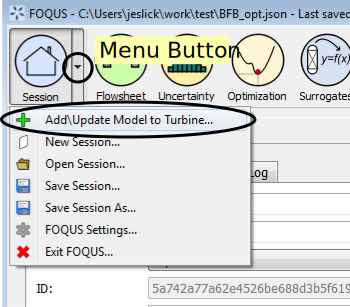
\includegraphics[scale=0.55]{Chapt_flowsheet/figs/menu_upload}
		\caption{Open Upload to Turbine Dialog}
		\label{fig.tut.opt.menu.upload}
	\end{center}
\end{figure}
\begin{figure}[H]
	\begin{center}
		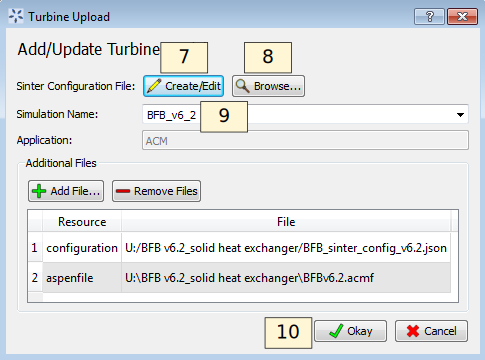
\includegraphics[scale=0.55]{Chapt_flowsheet/figs/upload}
		\caption{Upload to Turbine Dialog}
		\label{fig.tut.opt.upload}
	\end{center}
\end{figure}
The next step is to create the flowsheet.  Figure \ref{fig.tut.opt.drawFlowsheet} illustrates the steps to draw the flowsheet.
\begin{enumerate}
	\setcounter{enumi}{11}
	\item Click \bu{Flowsheet} at the top of the Home window.
	\item Click \bu{Add Node mode}.
	\item Add two nodes to the flowsheet. Name the first node ``BFB'' and the second node ``cost''.
	\item Click \bu{Add Edge mode}.
	\item Click the BFB node followed by the cost node.
	\item Click \bu{Selection mode} and select the BFB node.
	\item Click \bu{Toggle Node Editor}.  The Node Editor displays as illustrated in Figure \ref{fig.tut.opt.nodeEditor}.
\end{enumerate}
\begin{figure}[H]
	\begin{center}
		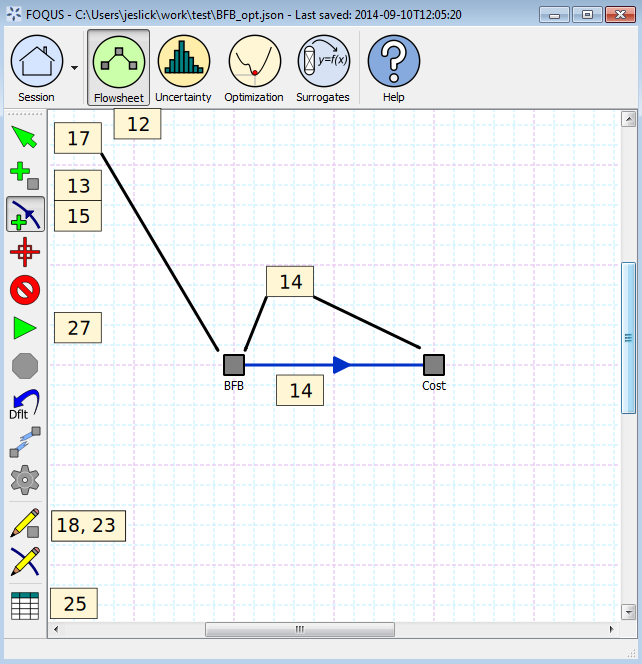
\includegraphics[scale=0.55]{Chapt_flowsheet/figs/flowsheetDraw}
		\caption{Flowsheet Editor}
		\label{fig.tut.opt.drawFlowsheet}
	\end{center}
\end{figure}
Each node must be assigned the appropriate simulation. Use the Node Editor to set the simulation type and the simulation name from simulation uploaded to Turbine. The Node Editor is illustrated in Figure \ref{fig.tut.opt.nodeEditor}
\begin{enumerate}
	\setcounter{enumi}{18}
	\item Under \bu{Model} and \bu{Type}, set the simulation \textbf{\underline{Type}} to Turbine. This indicates that the simulation is to be run with Turbine.
	\item Under \bu{Model}, set the simulation of the BFB node to BFB\_v6\_2.
	\item The \textbf{\underline{Variables}} and \textbf{\underline{Settings}} are automatically populated from the SimSinter configuration file. Variable values, \textbf\underline{{Min/Max}}, and descriptions can be changed; however, for this problem, the values taken from the SimSinter configuration should not be changed.
	\item Repeat the process for the cost node, assigning it the BFB\_v6\_2\_cost simulation.
\end{enumerate}
\begin{figure}[H] 
	\begin{center} 
		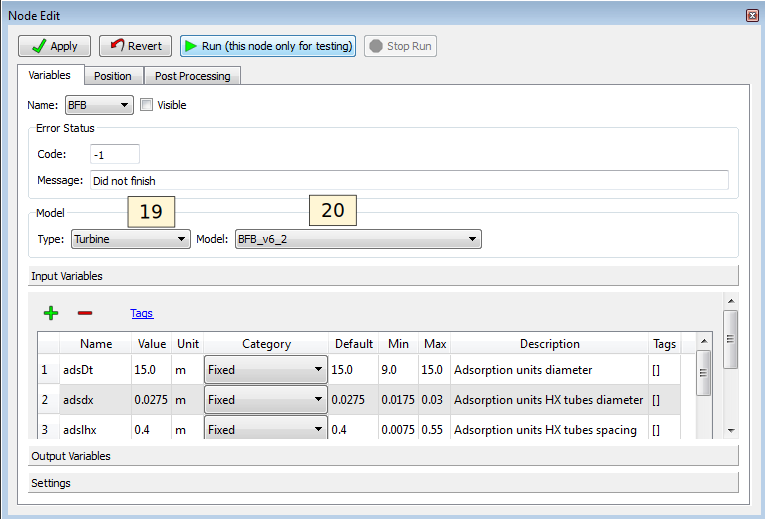
\includegraphics[scale=0.55]{Chapt_flowsheet/figs/nodeEditor}
		\caption{Node Editor}
		\label{fig.tut.opt.nodeEditor}
	\end{center}
\end{figure}
The connections between variables in the BFB simulation and the cost estimation spreadsheet must be set, so that required information can be transferred from the BFB simulation to the cost simulation.

\begin{enumerate}
	\setcounter{enumi}{22}
	\item Click \bu{Toggle Node Editor} to hide the Node Editor (Figure \ref{fig.tut.opt.drawFlowsheet}).
	\item Select the edge on the flowsheet with the \bu{Selection} tool.
	\item Click \bu{Toggle Edge Editor} to show the Edge Editor. The Edge Editor is shown in Figure \ref{fig.tut.opt.edgeEditor}.
	\item For convenience, all of the variables that should be connected from the ACM model to the Excel spreadsheet have been given the same names in their SimSinter configuration files. To connect the variables click \bu{Auto} in the Edge Editor.  \bu{Auto} connects variables of the same name. Since this is often not desired, the \bu{Auto} button should be used carefully. There should be 46 connected variables.
\end{enumerate}

\begin{figure}[H] 
	\begin{center} 
		
\includegraphics[scale=0.55]{Chapt_flowsheet/figs/edgeEditor}
		\caption{Edge Editor}
		\label{fig.tut.opt.edgeEditor}
	\end{center}
\end{figure}

The flowsheet should now be ready to run. Test the flowsheet by executing a single evaluation before setting up the optimization problem.

\begin{enumerate}
	\setcounter{enumi}{26}
	\item Click \bu{Run} in the Flowsheet Editor (Figure \ref{fig.tut.opt.drawFlowsheet}).
	\item The flowsheet may take a few minutes to run.  The BFB simulation takes a significant amount of time to open in ACM. While running optimization, the evaluations take less time because the simulation remains opened. The simulation should complete successfully. A message box displays when the simulation is done. The status bar also indicates the simulation is running.
	\item While the simulation is running, \bu{Stop} is enabled.
	\item Once the simulation runs successfully, \textbf{\underline{Save}} the FOQUS session again, and \textbf{keep it for use in later tutorials}.
\end{enumerate}
